\chapter{HMMER}

\section{HMMER简介}

\begin{quotation}
    HMMER is used for searching sequence databases for sequence homologs, and for making sequence alignments. It implements methods using probabilistic models called profile hidden Markov models (profile HMMs).

    HMMER is often used together with a profile database, such as Pfam or many of the databases that participate in Interpro. But HMMER can also work with query sequences, not just profiles, just like BLAST. For example, you can search a protein query sequence against a database with phmmer, or do an iterative search with jackhmmer.

    HMMER is designed to detect remote homologs as sensitively as possible, relying on the strength of its underlying probability models. In the past, this strength came at significant computational expense, but as of the new HMMER3 project, HMMER is now essentially as fast as BLAST.

    HMMER can be downloaded and installed as a command line tool on your own hardware, and now it is also more widely accessible to the scientific community via new search servers at the European Bioinformatics Institute.

    \textit{http://hmmer.org/}

\end{quotation}

\section{HMMER网站的四种搜索方法}

\subsection{phmmer}
\textit{single protein sequence against protein sequence database}

使用蛋白质序列在蛋白质数据库中搜索

phmmer is used to search one or more query protein sequences against a protein sequence database. For each query sequence in seqfile, use that sequence to search the target database of sequences in seqdb, and output ranked lists of the sequences with the most significant matches to the query.

\begin{quotation}

    \textit{https://www.mankier.com/1/phmmer}

\end{quotation}

\subsection{hmmscan}
\textit{single protein sequence against profile HMM library (Pfam,CATH-Gene3D,PIRSF Superfamily and TIGRFAMs).}

序列搜序列谱(以HMM构建的序列谱)

hmmscan is used to search protein sequences against collections  of protein profiles. For each sequence in seqfile, use that query sequence to search the target database of profiles in hmmdb, and output ranked lists of the profiles with the most significant matches to the sequence.

\begin{quotation}

    \textit{https://www.mankier.com/1/hmmscan}

\end{quotation}


\subsection{hmmsearch}
\textit{either multiple sequence alignment or profile HMM against protein sequence database.}

序列谱搜序列

hmmsearch is used to search one or more profiles against a sequence database. For each profile in hmmfile, use that query profile to search the target database of sequences in seqdb, and output ranked lists of the sequences with the most significant matches to the profile.

\begin{quotation}

    \textit{https://www.mankier.com/1/hmmsearch}

\end{quotation}

\subsection{jackhmmer}
\textit{iterative searches. lnitiated with a single sequence, a profileHMM or a multiple sequence alignment against a target sequence database.}

迭代搜索

jackhmmer iteratively searches each query sequence in seqfile against the target sequence(s) in seqdb. The first iteration is identical to a phmmer search. For the next iteration, a multiple alignment of the query together with all target sequences satisfying  inclusion thresholds is assembled, a profile is constructed from this alignment (identical to using hmmbuild on the alignment), and profile search of the seqdb is done (identical to an hmmsearch with the profile).

\begin{quotation}
    \textit{https://www.mankier.com/1/jackhmmer}
\end{quotation}

\section{Hmmer的网站使用实例:以jackhmmer为例}

WSL提供了一个完整的Linux内核,但它不是一个虚拟机。相反,WSL提供了一个Linux系统调用兼容层,以便可以在Windows上运行原生Linux二进制文件。这意味着您可以在Windows上运行Linux命令行工具、脚本和应用程序,而无需使用虚拟机或双引导设置。


(1)在uniprot上下载目标蛋白序列

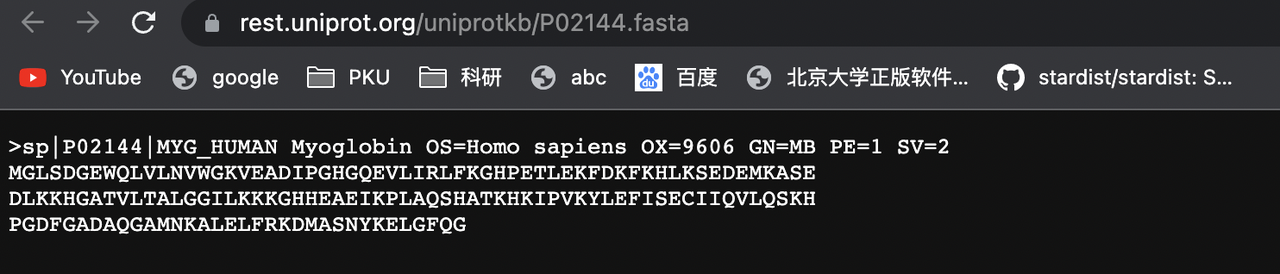
\includegraphics[width=0.8\textwidth]{./image/gdk/7.4.1.png}

(2)登陆hmmer网址-search-jackhmmer,输入序列

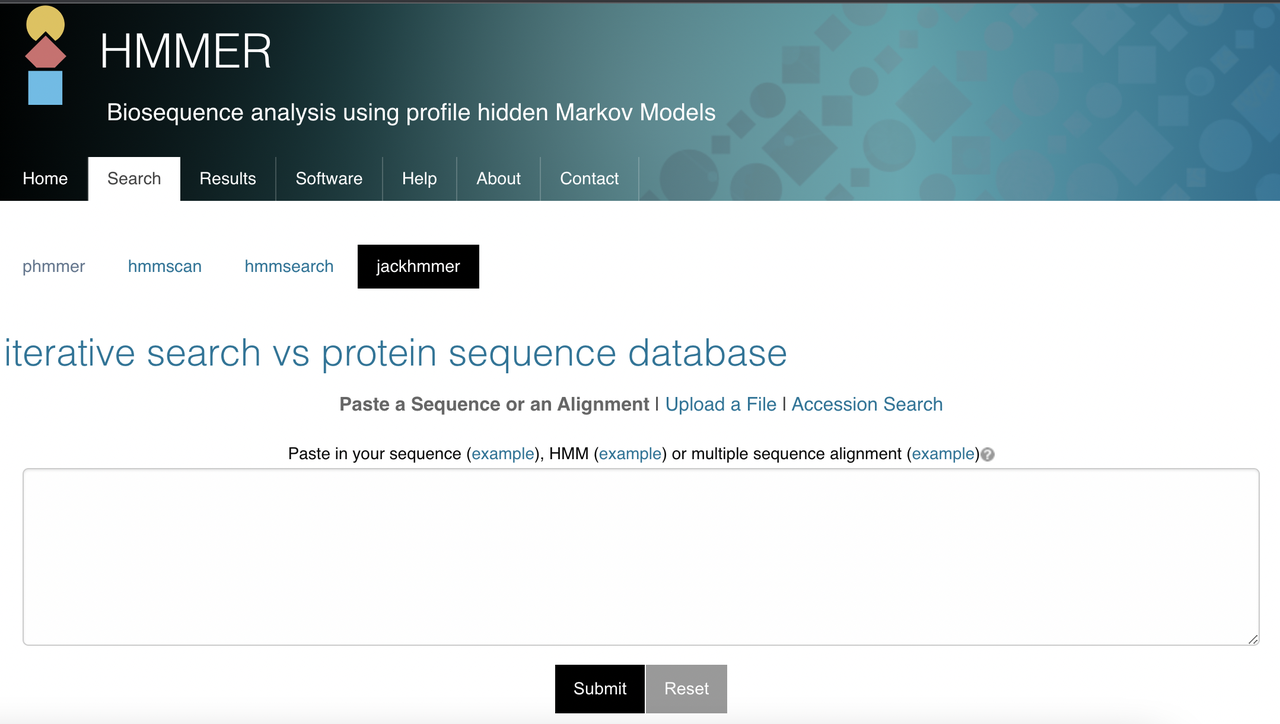
\includegraphics[width=0.8\textwidth]{./image/gdk/7.4.2.png}

(3)选择比对数据库与评估标准

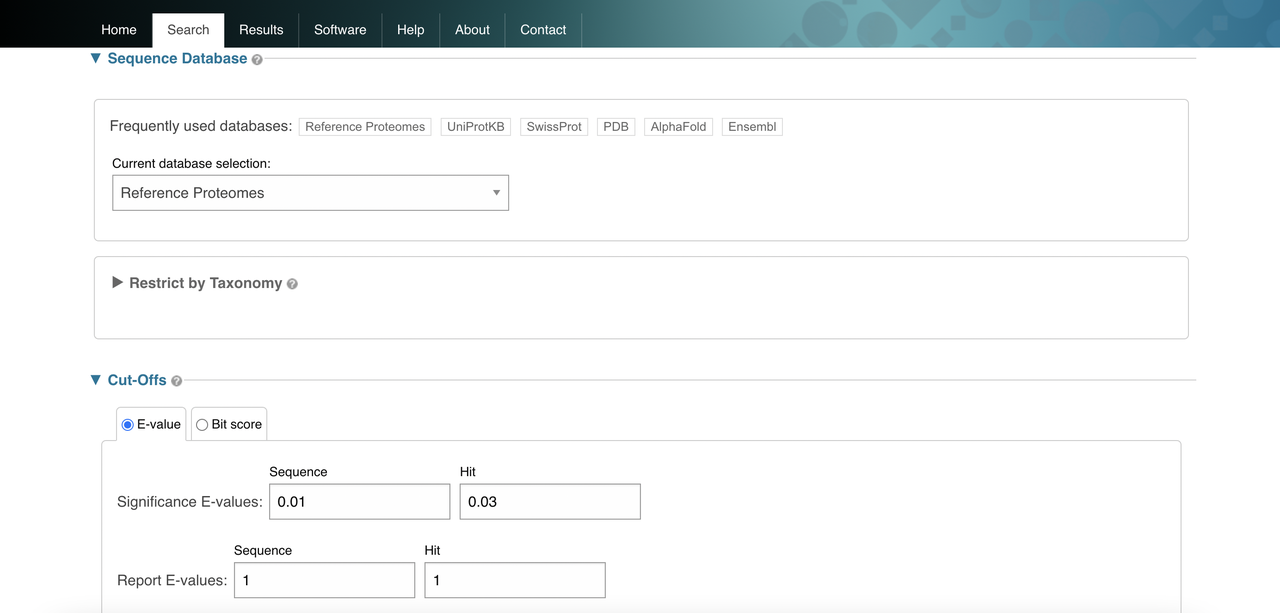
\includegraphics[width=0.8\textwidth]{./image/gdk/7.4.3.png}

(4)得到比对结果

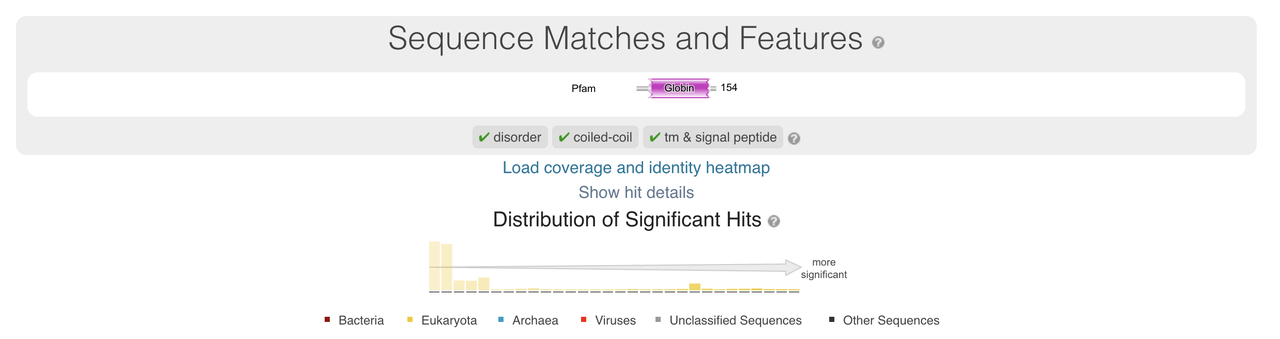
\includegraphics[width=0.8\textwidth]{./image/gdk/7.4.4.png}

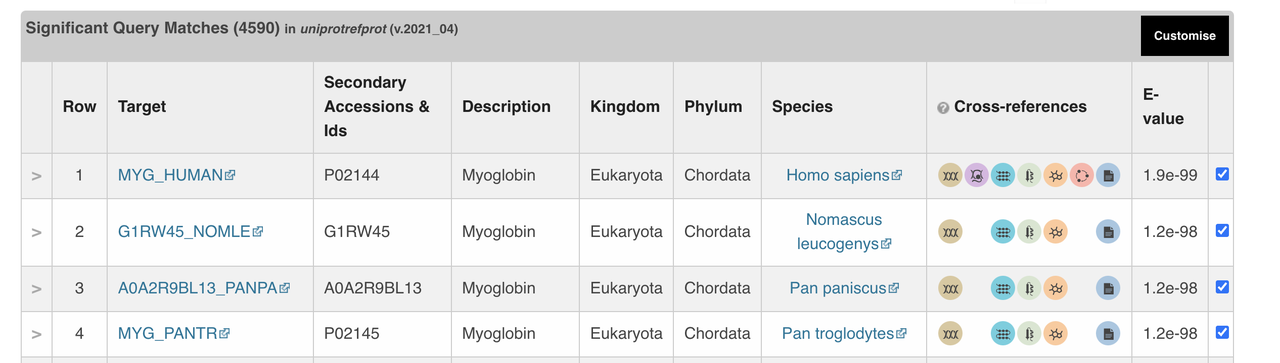
\includegraphics[width=0.8\textwidth]{./image/gdk/7.4.5.png}


(5)右上角customise可以选择需要列举的属性

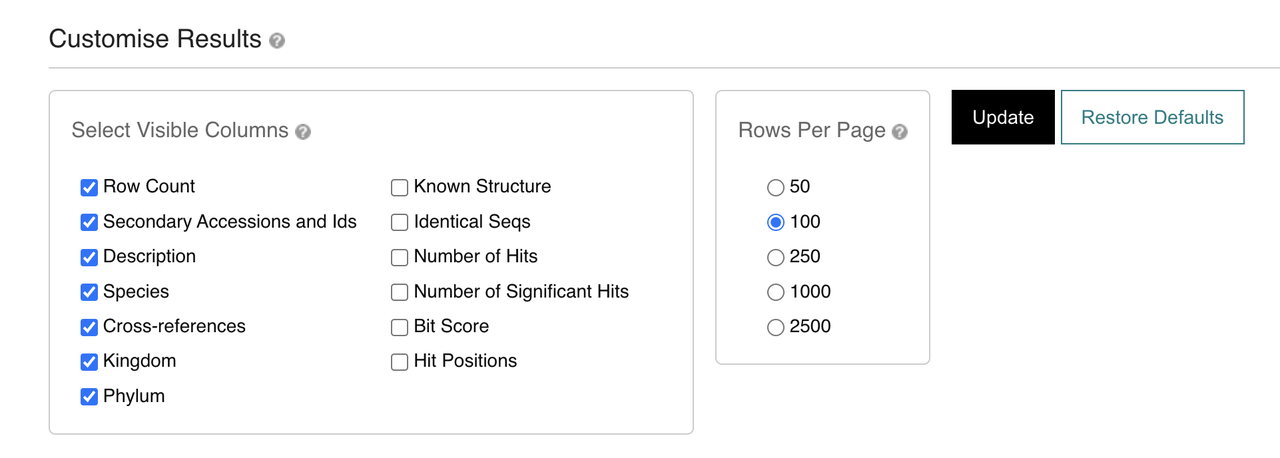
\includegraphics[width=0.8\textwidth]{./image/gdk/7.4.6.png}

(6)点击序列可以看到详细的对比情况

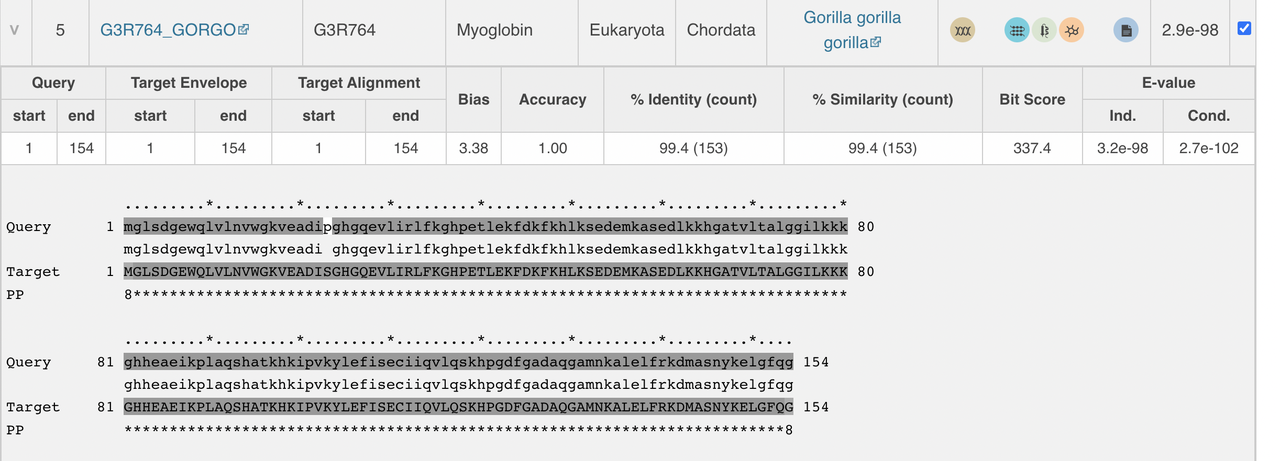
\includegraphics[width=0.8\textwidth]{./image/gdk/7.4.7.png}

(7)点击taxonomy可以得到分类图,其中的每一个节点都可以当作筛选的标准

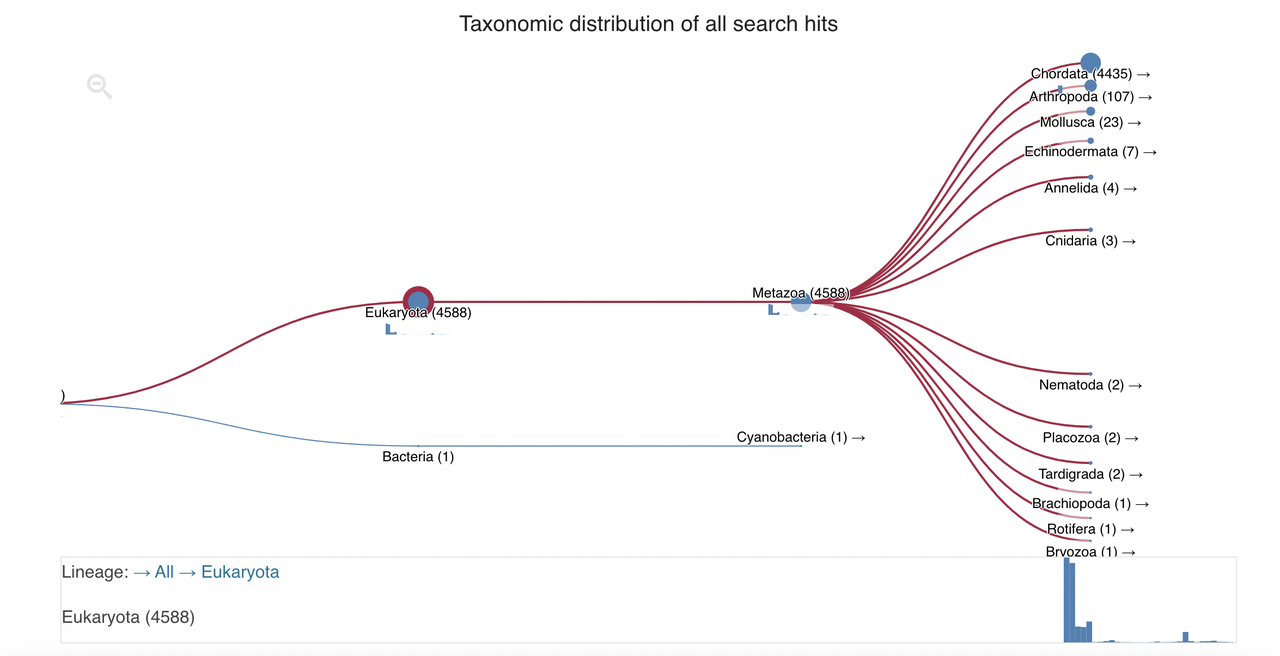
\includegraphics[width=0.8\textwidth]{./image/gdk/7.4.8.png}

(8)点击一轮迭代的右下角的“next iteration”,进行下一轮的迭代

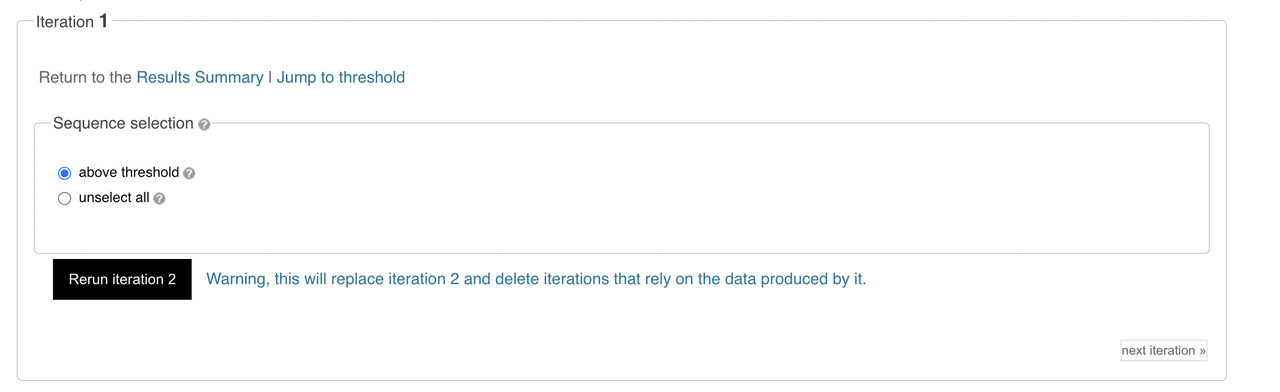
\includegraphics[width=0.8\textwidth]{./image/gdk/7.4.9.png}

(9)得到E-value极低的比对结果,此外还能得到Model Position图

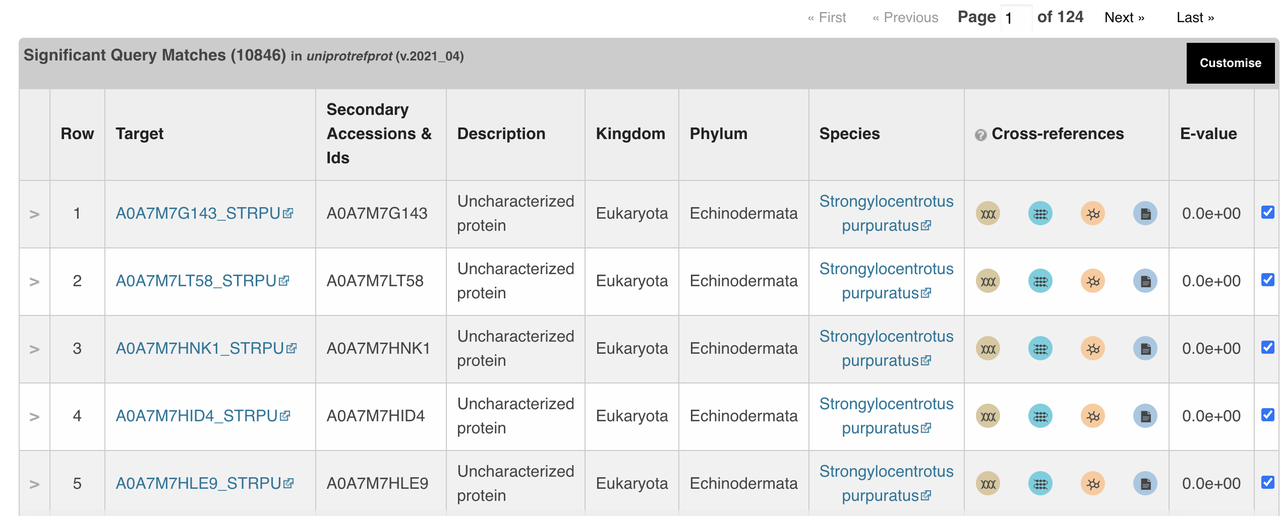
\includegraphics[width=0.8\textwidth]{./image/gdk/7.4.10.png}

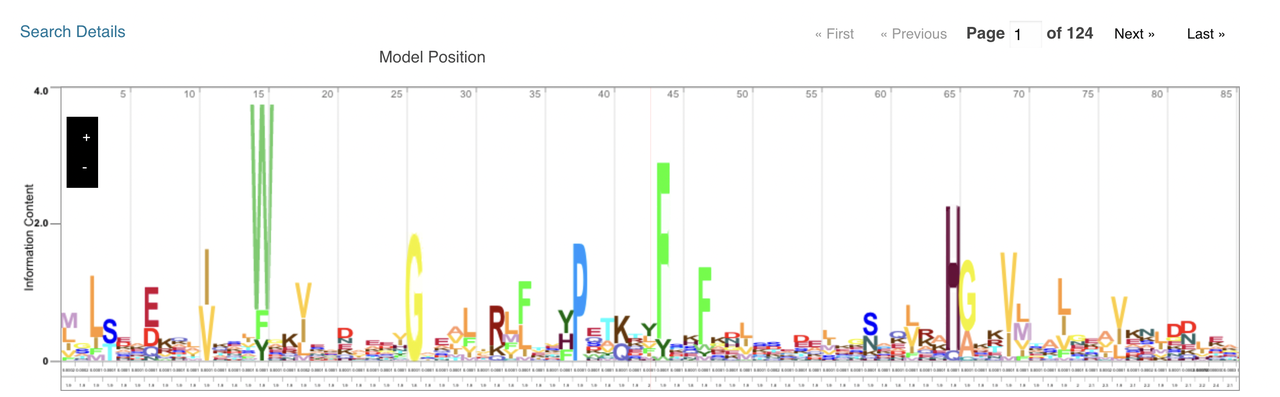
\includegraphics[width=0.8\textwidth]{./image/gdk/7.4.11.png}

\section{在python上使用HMMER}

将下列代码引入python中,并下载HMMER对应的数据库

\begin{lstlisting}
    import pyhmmer
    with pyhmmer.easel.SequenceFile("pyhmmer/tests/data/seqs/938293.PRJEB85.HG003687.faa",                                      digital=True) as seq_file:
        sequences = list(seq_file)
    with pyhmmer.plan7.HMMFile("pyhmmer/tests/data/hmms/txt/t2pks.hmm") as hmm_file:
        for hits in pyhmmer.hmmsearch(hmm_file, sequences, cpus=4):
            print(f"HMM {hits.query_name.decode()} found {len(hits)} hits in the target sequences")

\end{lstlisting}